\documentclass{beamer}
\usetheme{Madrid}
\usecolortheme{default}

\title[DeepBait]
{DeepBait: Article-Conditioned Clickbait Headline Generation}

\subtitle{Group 23}

\author[Group 23]
{Irys Zhang\inst{1} \and Jiangchuan Yu\inst{2} \and Yushun Tang\inst{3}}

\institute[ ]
{
  \inst{1}%
  Department of Electrical and Computer Engineering
}

\date[AplDL]
{Applied Deep Learning -- Winter 2026}

\logo{
\includegraphics[height=0.8cm]{logo_uoft}}

\definecolor{uoftblue}{RGB}{6,41,88}
\setbeamercolor{titlelike}{bg=uoftblue}
\setbeamerfont{title}{series=\bfseries}

\usepackage{booktabs}
\usepackage{tikz}
\usetikzlibrary{arrows.meta, positioning}

\begin{document}

\frame{\titlepage}


%% ============================================================
%% SLIDE 1 — Problem & Motivation
%% ============================================================
\begin{frame}
\frametitle{Problem \& Motivation}

\begin{block}{The Problem}
Most clickbait research focuses on \alert{detection} (classification).\\
Generating clickbait headlines \textit{conditioned on article content} is underexplored.
\end{block}

\vspace{0.3cm}

\textbf{Our Goal:} Given a news article, automatically generate a clickbait-style headline that relates to the article's content.

\vspace{0.3cm}

\textbf{Why it matters:}
\begin{itemize}
    \item Understanding how clickbait exploits article content
    \item Generating adversarial samples for improving clickbait detectors
    \item Exploring conditional text generation with limited data
\end{itemize}

\end{frame}


%% ============================================================
%% SLIDE 2 — Architecture & Approach
%% ============================================================
\begin{frame}
\frametitle{Model Architecture}

\begin{center}
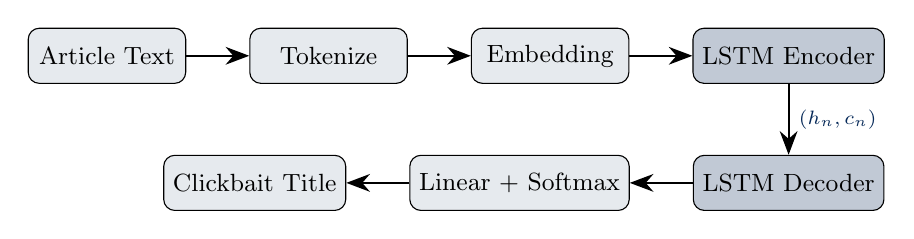
\begin{tikzpicture}[
    node distance=0.5cm and 0.8cm,
    box/.style={draw, rounded corners, minimum height=0.7cm, minimum width=2.0cm, font=\small, fill=uoftblue!10},
    arr/.style={-{Stealth[length=3mm]}, thick},
    lbl/.style={font=\scriptsize, text=uoftblue}
]
    \node[box] (input) {Article Text};
    \node[box, right=of input] (tok) {Tokenize};
    \node[box, right=of tok] (emb) {Embedding};
    \node[box, right=of emb, fill=uoftblue!25] (enc) {LSTM Encoder};

    \node[box, below=0.9cm of enc, fill=uoftblue!25] (dec) {LSTM Decoder};
    \node[box, left=of dec] (fc) {Linear + Softmax};
    \node[box, left=of fc] (out) {Clickbait Title};

    \draw[arr] (input) -- (tok);
    \draw[arr] (tok) -- (emb);
    \draw[arr] (emb) -- (enc);
    \draw[arr] (enc) -- node[right, lbl] {$(h_n, c_n)$} (dec);
    \draw[arr] (dec) -- (fc);
    \draw[arr] (fc) -- (out);
\end{tikzpicture}
\end{center}

\vspace{0.15cm}

\begin{columns}[T]
\begin{column}{0.48\textwidth}
\textbf{Seq2Seq LSTM}
\begin{itemize}
    \item Embedding: 128-d
    \item Hidden: 256-d, 2 layers
    \item Teacher forcing (train)
    \item Temperature sampling (inference)
\end{itemize}
\end{column}
\begin{column}{0.48\textwidth}
\textbf{BART Baseline (Exp 3)}
\begin{itemize}
    \item Fine-tune \texttt{bart-large-cnn}
    \item Already trained on summarisation
    \item Adapts style $\rightarrow$ clickbait
    \item 406M parameters
\end{itemize}
\end{column}
\end{columns}

\end{frame}


%% ============================================================
%% SLIDE 3 — Experiments & Results
%% ============================================================
\begin{frame}
\frametitle{Experiments \& Results}

\textbf{Data:} Kaggle Clickbait (3,724 pairs) + Webis-17 (4,696 pairs) $=$ \alert{8,420 total}; pretrain on CNN/DailyMail (${\sim}307$K pairs)

\vspace{0.2cm}

\begin{table}[h]
\centering
\small
\begin{tabular}{@{}llcc@{}}
\toprule
\textbf{Exp} & \textbf{Method} & \textbf{Best Val Loss} & \textbf{Val PPL} \\
\midrule
1 & Direct Seq2Seq (Webis+Kaggle) & 6.278 & 533 \\
2a & Pretrain on CNN/DailyMail     & 5.251 & 191 \\
2b & + Finetune on clickbait       & 5.216 & 184 \\
3 & BART fine-tune                 & \alert{2.038} & \alert{7.7} \\
\bottomrule
\end{tabular}
\end{table}

\vspace{0.15cm}

\begin{alertblock}{Key Finding}
Transfer learning dominates: BART achieves \textbf{PPL 7.7} vs.\ LSTM's best of 184. Even within LSTMs, pretrain $\rightarrow$ finetune cuts perplexity by \textbf{65\%} over direct training (184 vs.\ 533).
\end{alertblock}

\end{frame}


%% ============================================================
%% SLIDE 4 — Conclusion & Future Work
%% ============================================================
\begin{frame}
\frametitle{Conclusion \& Future Work}

\begin{block}{Takeaways}
\begin{enumerate}
    \item Article-conditioned generation is far more meaningful than seed-phrase LMs
    \item Data augmentation (Webis-17) and two-stage training are critical for small-data seq2seq
    \item BART fine-tuning achieves \textbf{PPL 7.7}, vastly outperforming the LSTM (PPL 184)
\end{enumerate}
\end{block}

\vspace{0.3cm}

\textbf{Future Work:}
\begin{itemize}
    \item Add \textbf{attention mechanism} to let the decoder focus on relevant article segments
    \item Replace greedy / random sampling with \textbf{beam search}
    \item Compare BART vs.\ LSTM fluency via \textbf{human evaluation}
    \item Evaluate using \textbf{ROUGE / BERTScore} against real clickbait headlines
\end{itemize}

\end{frame}


\end{document}
